\documentclass{article}%
\usepackage[T1]{fontenc}%
\usepackage[utf8]{inputenc}%
\usepackage{lmodern}%
\usepackage{textcomp}%
\usepackage{lastpage}%
\usepackage[head=40pt,margin=0.5in,bottom=0.6in]{geometry}%
\usepackage{graphicx}%
%
\title{\textbf{Liberaron al periodista Isnardo Bravo}}%
\author{El Nacional Web}%
\date{24/09/2018}%
%
\begin{document}%
\normalsize%
\maketitle%
\textbf{URL: }%
http://www.el{-}nacional.com/noticias/sociedad/liberaron{-}periodista{-}isnardo{-}bravo\_253038\newline%
%
\textbf{Periodico: }%
EN, %
ID: %
253038, %
Seccion: %
Sociedad\newline%
%
\textbf{Palabras Claves: }%
NO\_TIENE\newline%
%
\textbf{Derecho: }%
1.2%
, Otros Derechos: %
NO\_TIENE%
, Sub Derechos: %
1.2.1.3%
\newline%
%
\textbf{EP: }%
SI\newline%
\newline%
%
\textbf{\textit{El comunicador social fue detenido en el Aeropuerto Internacional Simón Bolívar donde se le informó que tiene prohibición para salir del país ~}}%
\newline%
\newline%
%
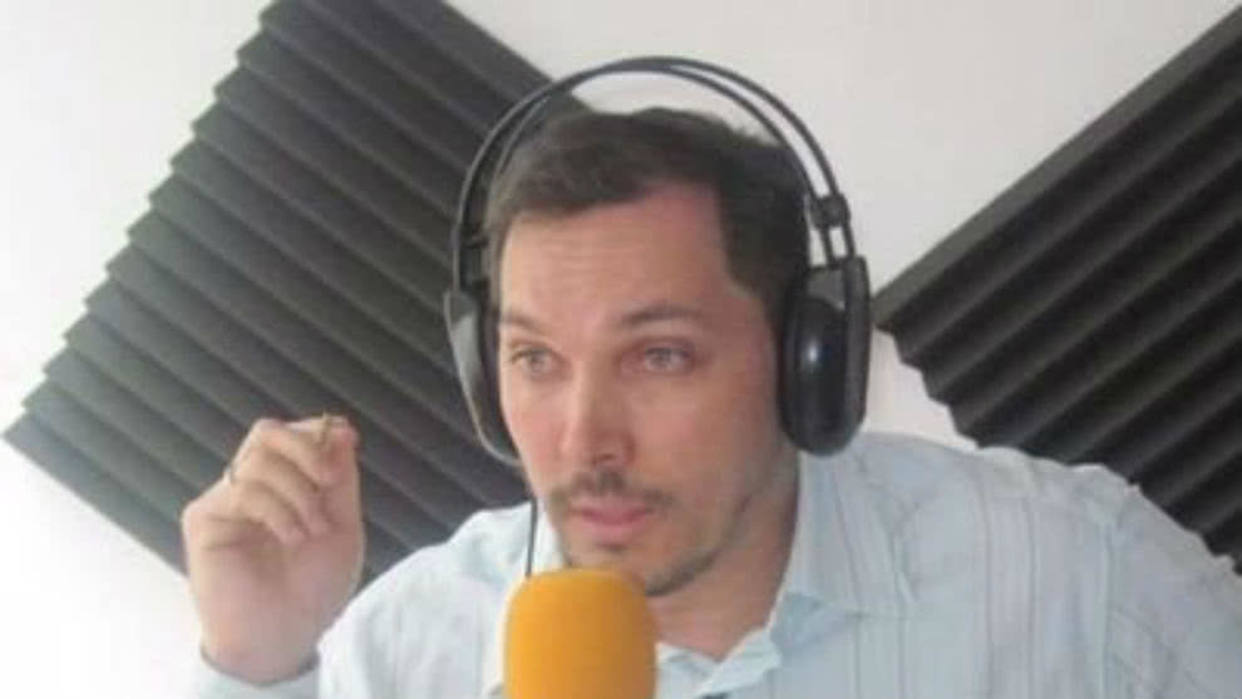
\includegraphics[width=300px]{163.jpg}%
\newline%
%
El periodista Isnardo Bravo fue liberado luego de estar retenido por más de ocho horas.%
\newline%
%
El comunicador social primero estuvo detenido en la oficina del~Servicio Administrativo de Identificación, Migración y Extranjería del Aeropuerto Internacional Simón Bolívar y luego en la sede de la Dirección General de Contrainteligencia Militar en Boleíta, municipio Sucre en el estado Miranda.%
\newline%
%
El periodista fue retenido en el aeropuerto~donde se presuntamente se le informó que tiene prohibición de salida~del país, por lo que retuvieron su pasaporte.%
\newline%
%
Bravo, quien se disponía a salir del país junto a su hija de 11 años de edad cuando fue detenido, recientemente renovó su pasaporte en el Saime sin ningún problema, informó la abogada Theresly Malave.%
\newline%
%
\end{document}